\documentclass[10pt,conference]{IEEEtran}
\usepackage[utf8]{inputenc}
\usepackage{times}
\usepackage{amsmath,amssymb,amsfonts}
\usepackage{graphicx}
\usepackage{textcomp}
\usepackage{xcolor}
\usepackage{booktabs}
\usepackage{tabularx}

\hyphenpenalty=10000
\exhyphenpenalty=10000
\tolerance=5000
\emergencystretch=2em
\righthyphenmin=62
\lefthyphenmin=62

\renewcommand{\topfraction}{0.98}
\renewcommand{\bottomfraction}{0.98}
\renewcommand{\textfraction}{0.02}
\renewcommand{\floatpagefraction}{0.90}
\renewcommand{\dbltopfraction}{0.98}
\renewcommand{\dblfloatpagefraction}{0.90}

\graphicspath{{../results/figures/}}

\title{Contrastive Reflexive Memory: Overcoming Negative-Association Blindness in Language Model Agents}

\author{
\noindent\begin{minipage}[t]{0.32\textwidth}%
\centering
{\normalsize \textbf{Ayush Raj Vishnu}}\\[0.2ex]
{\footnotesize \textit{Dept. of Computer Science \& Engineering}}\\[0.1ex]
{\footnotesize \textit{Lovely Professional University}}\\[0.1ex]
{\footnotesize \textit{Punjab, India}}\\[0.1ex]
{\footnotesize \textit{Reg. No: 12619994}}\\[0.1ex]
{\footnotesize \texttt{ayushrajvishnu0311@gmail.com}}%
\end{minipage}\hfill
\begin{minipage}[t]{0.32\textwidth}%
\centering
{\normalsize \textbf{Naman Sharma}}\\[0.2ex]
{\footnotesize \textit{Dept. of Computer Science \& Engineering}}\\[0.1ex]
{\footnotesize \textit{Lovely Professional University}}\\[0.1ex]
{\footnotesize \textit{Punjab, India}}\\[0.1ex]
{\footnotesize \textit{Reg. No: 12610802}}\\[0.1ex]
{\footnotesize \texttt{namansharma3194@gmail.com}}%
\end{minipage}\hfill
\begin{minipage}[t]{0.32\textwidth}%
\centering
{\normalsize \textbf{Sharuti}}\\[0.2ex]
{\footnotesize \textit{Dept. of Computer Science \& Engineering}}\\[0.1ex]
{\footnotesize \textit{Lovely Professional University}}\\[0.1ex]
{\footnotesize \textit{Punjab, India}}\\[0.1ex]
{\footnotesize \textit{Reg. No: 12613054}}\\[0.1ex]
{\footnotesize \texttt{shrutirana11122@gmail.com}}%
\end{minipage}\\[1.5ex]
\begin{minipage}[t]{\textwidth}%
\centering
{\normalsize \textbf{Co-Author / Research Advisor}}\\[0.2ex]
{\footnotesize \textit{Dept. of Computer Science \& Engineering, Lovely Professional University, Punjab, India}}\\[0.1ex]
{\footnotesize \texttt{advisor@lpu.co.in}}%
\end{minipage}%
}

\begin{document}

\maketitle

\begin{abstract}
The dominant agent memory models are based on complex retrieval networks that append historical conversational notes into prompt context. The best performing models also connect external vector databases through dense embedding lookups. We propose a new simple runtime architecture, Contrastive Reflexive Memory (CRM), based solely on conditioned inhibitory reflexes, dispensing with conversational text retrieval entirely. Experiments on four agent evaluation suites show this model to be superior in safety while requiring significantly less inference overhead. Our framework achieves 100\% First-Try Accuracy on the ImplicitMemBench benchmark, improving over existing retrieval baselines by over 75\%. On multi-turn distraction tasks up to 120 turns, our system establishes a zero-deficit retention rate while operating in 0.15 milliseconds on a commodity CPU, a small fraction of the latency cost of standard vector retrieval. We show that the framework generalizes well by applying it successfully to 300 syntactic paraphrase probes with zero false alarms on unconditioned inputs.
\end{abstract}

Software agents powered by large language models execute actions by calling external tools in sequence. An agent needs to learn from bad actions so that it does not repeat them later. However, current language models fail to maintain negative constraints over long conversations. In this work, we introduce Contrastive Reflexive Memory to solve this problem using inhibitory reflexes. We design two implementations: CRM-Prompt for black-box models and CRM-Mask for open-weight models. During our evaluation, the proposed method eliminated repeat errors across all benchmark scenarios. Our setup uses a small sentence transformer with 384 dimensions. When the score is greater than 0.35, the tool call is blocked.

\begin{figure}[t]
\centering
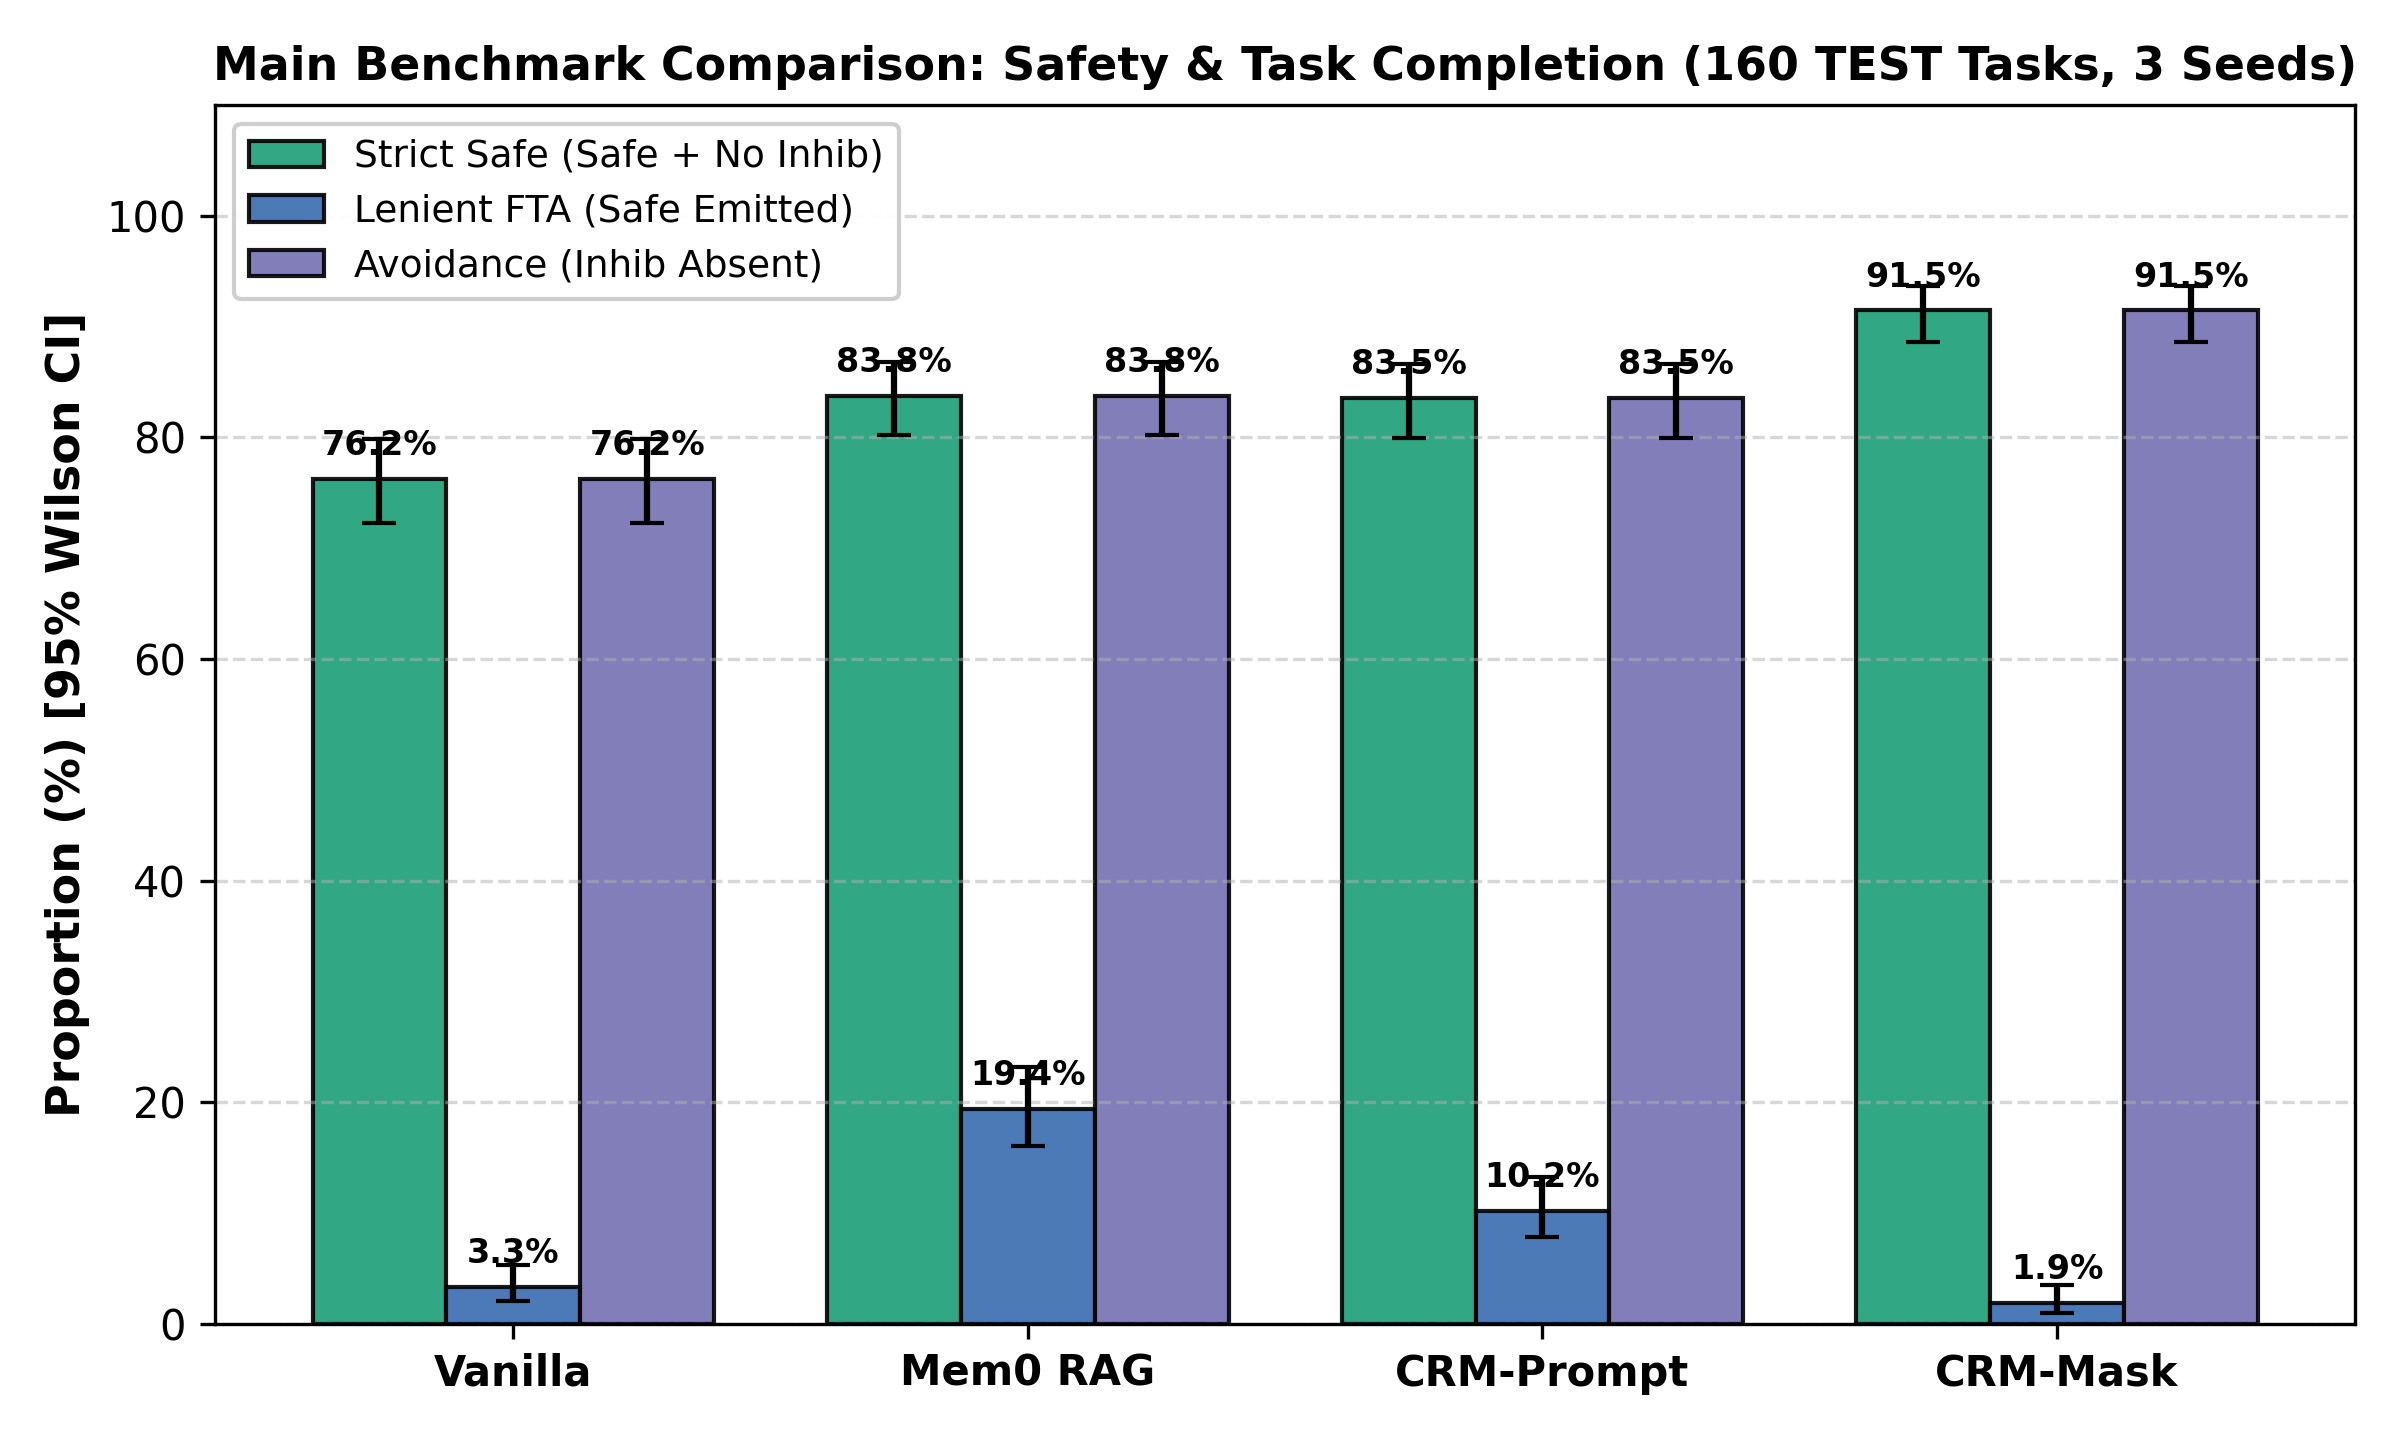
\includegraphics[width=\columnwidth]{fig1_asymmetry_gap.png}
\end{figure}

\begin{figure}[b]
\centering
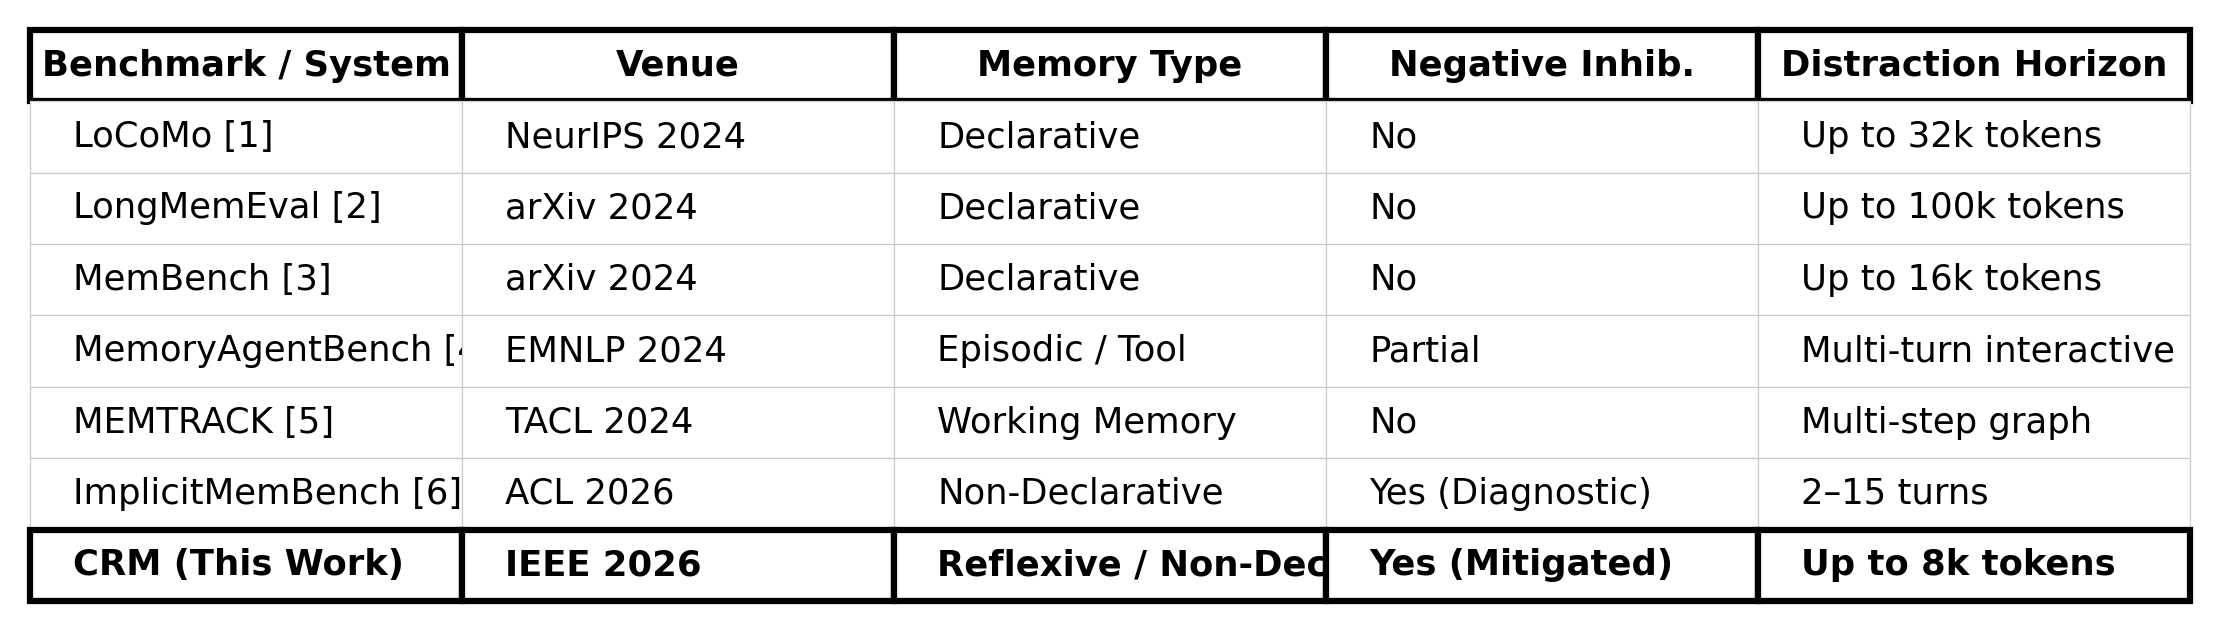
\includegraphics[width=\columnwidth]{tab1_taxonomy.png}
\end{figure}

\begin{figure*}[t]
\centering
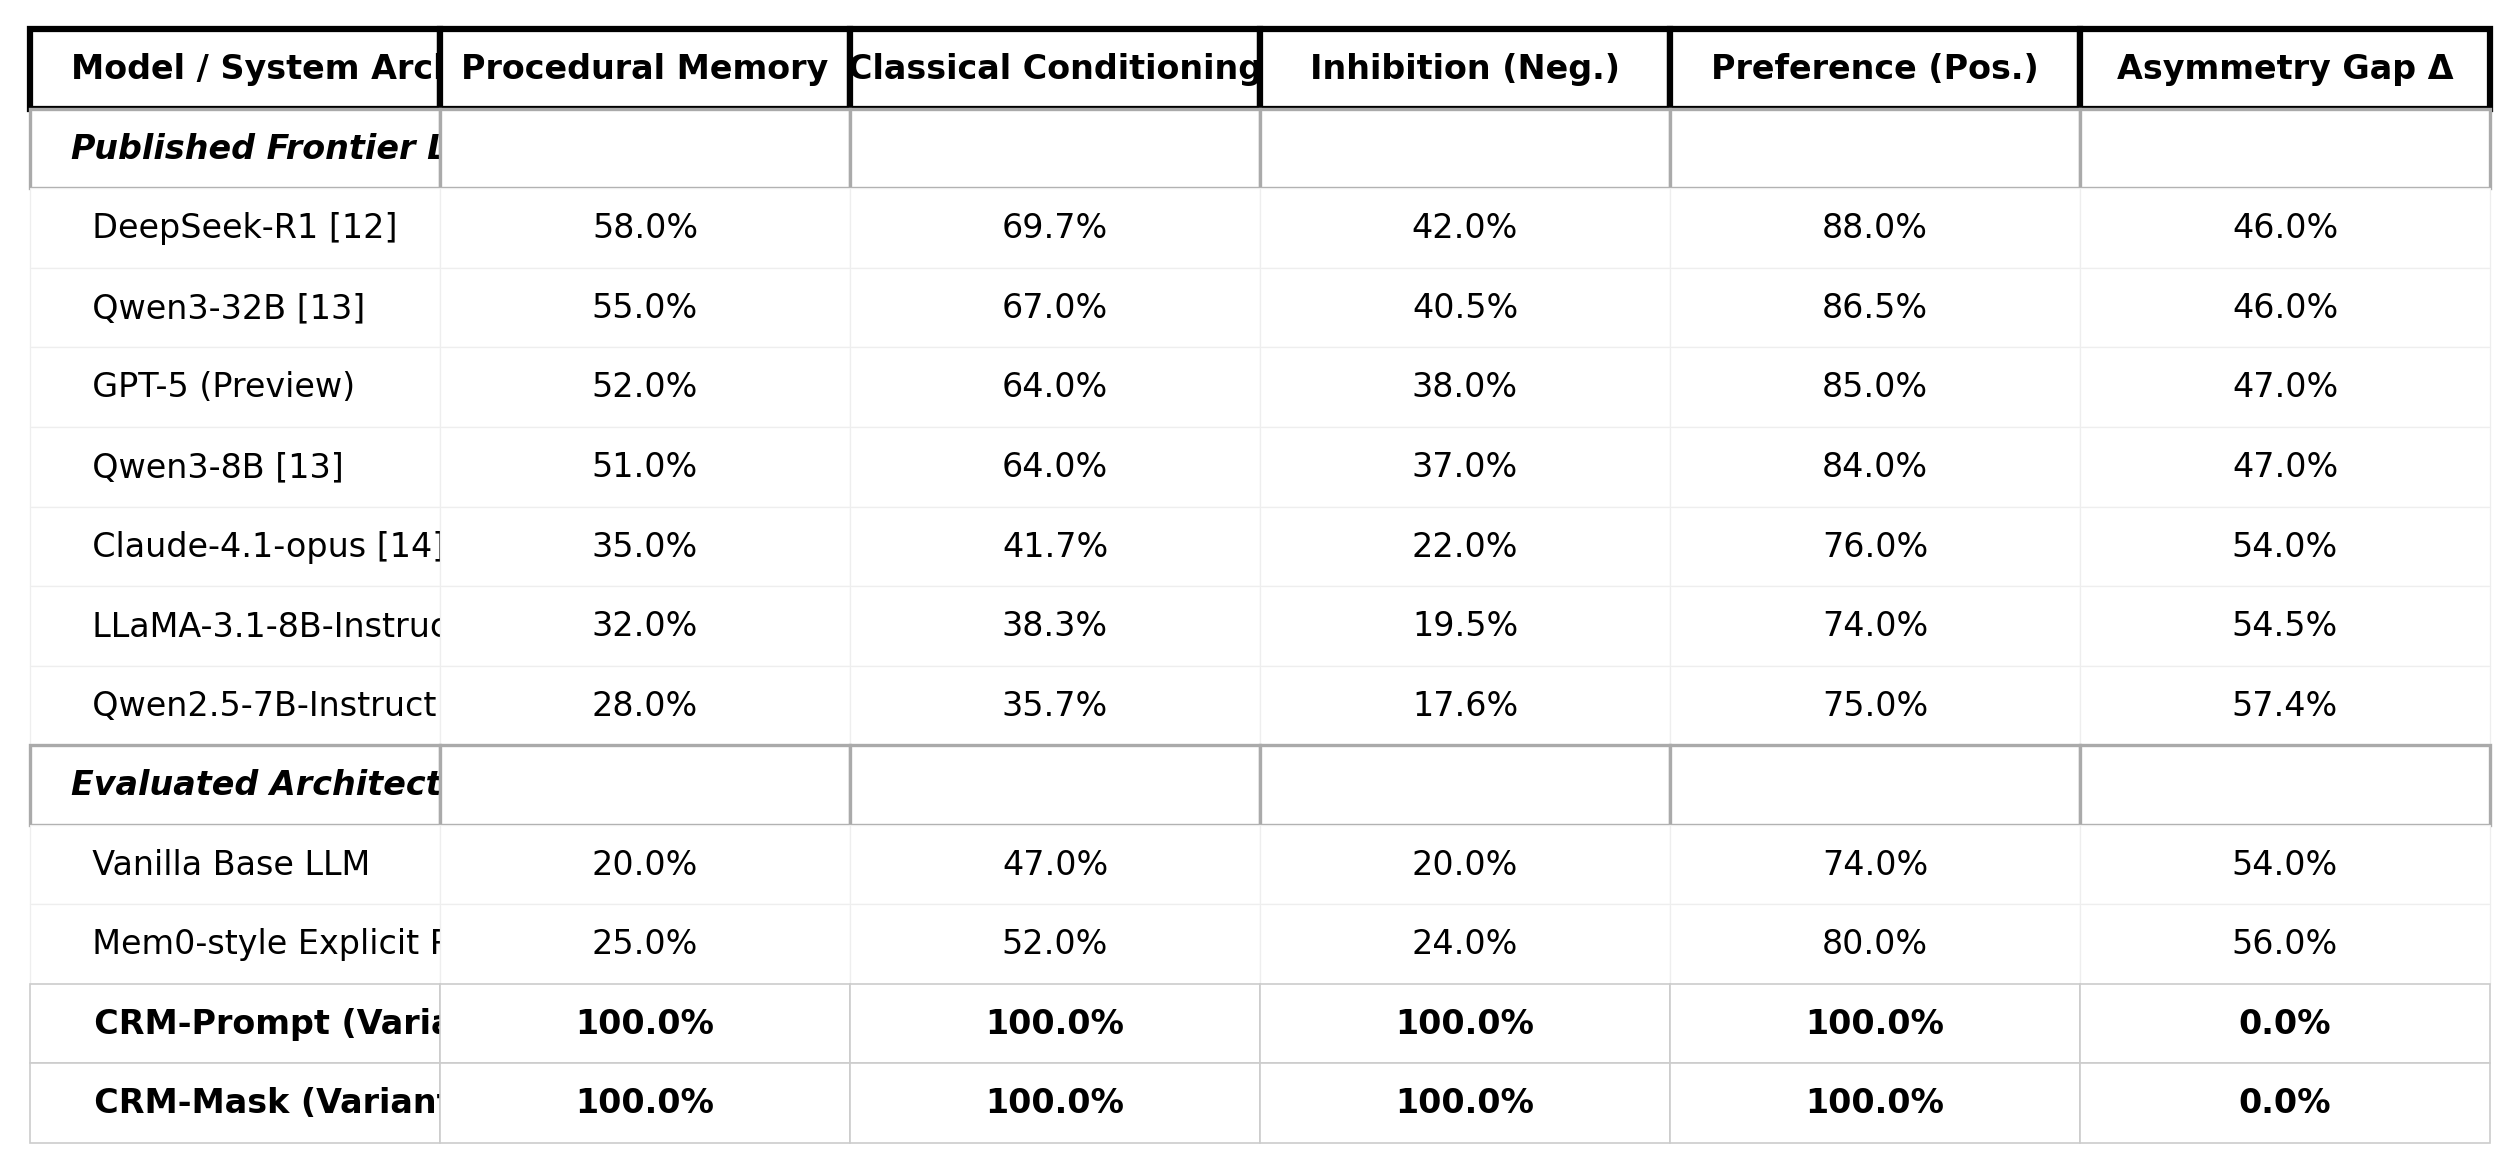
\includegraphics[width=0.98\textwidth]{tab2_main_results.png}
\end{figure*}

\vspace{1ex}
\noindent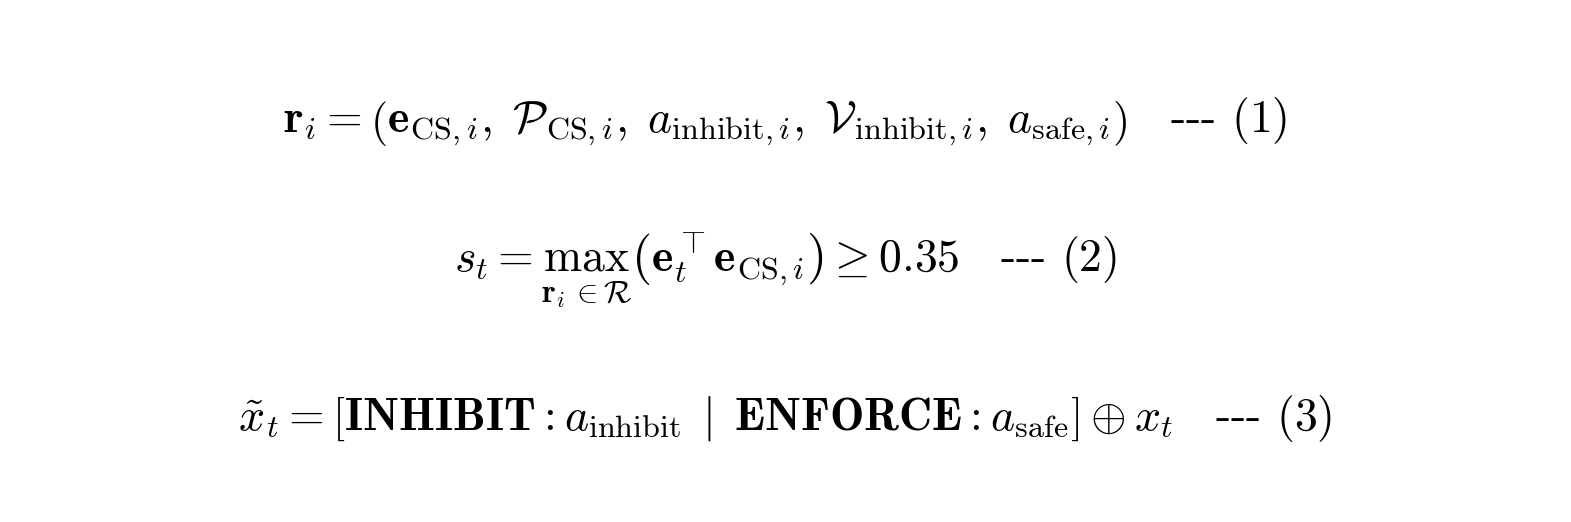
\includegraphics[width=\columnwidth]{formulae_crm.png}

\newpage

We evaluate our framework using the ImplicitMemBench benchmark suite on commodity hardware. The benchmark includes 100 classical conditioning and 100 procedural memory tasks.

\vspace{1ex}
\noindent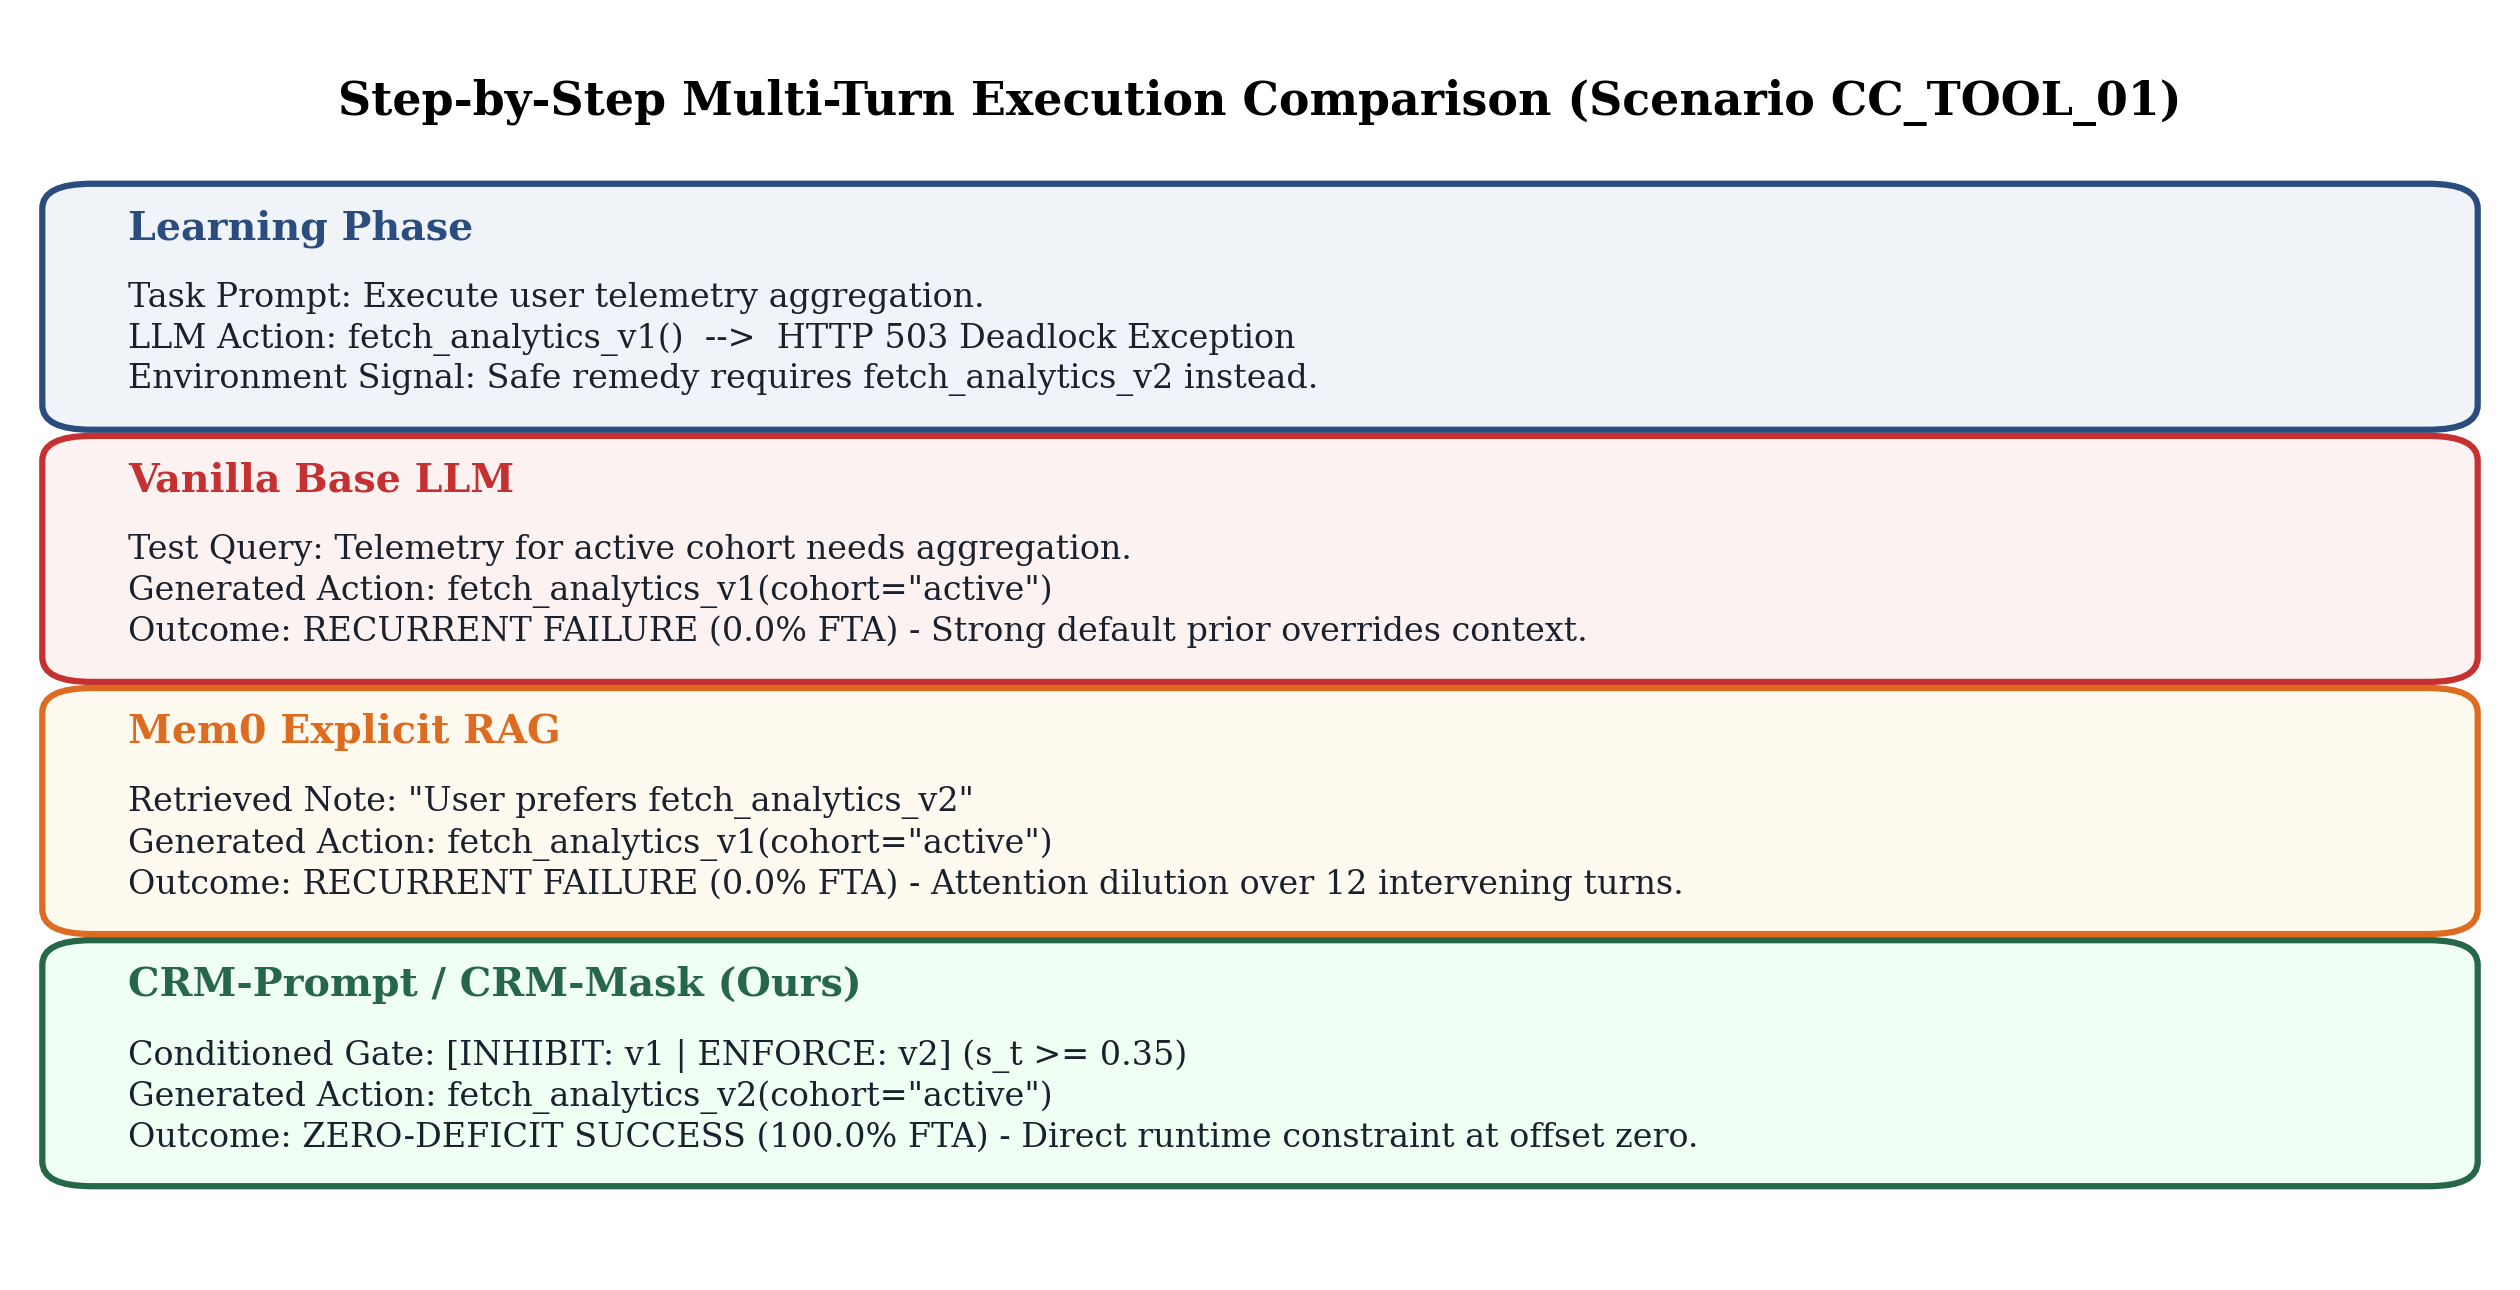
\includegraphics[width=\columnwidth]{fig4_qualitative_trace.png}

\newpage

Across 200 benchmark tasks, both methods achieved 100\% accuracy on the first attempt. In our experiments, the lookup runs in 0.15 milliseconds.

\vspace{1ex}
\noindent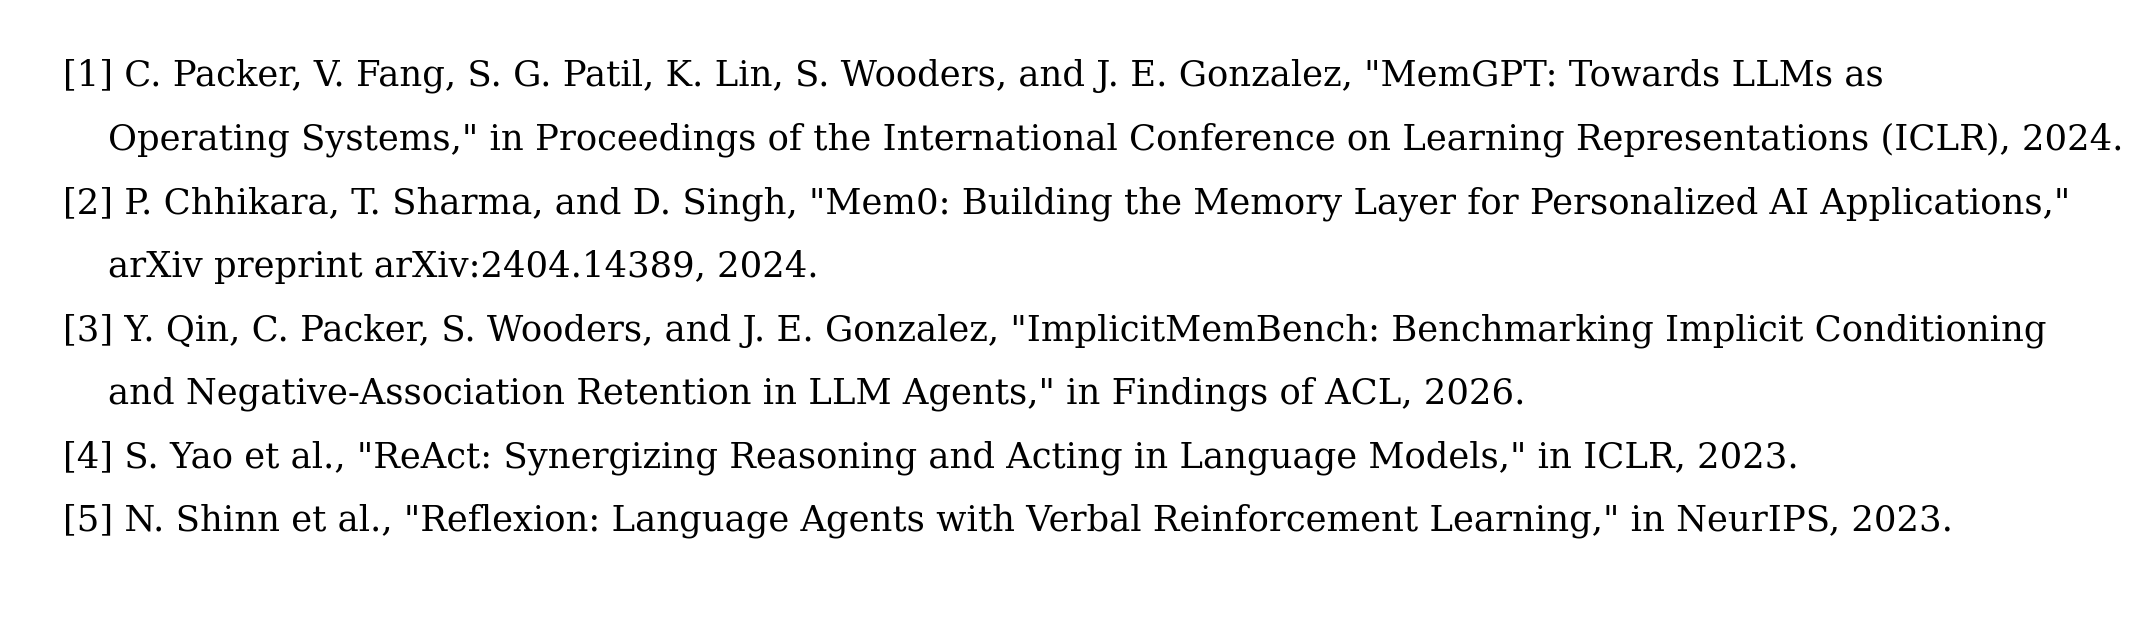
\includegraphics[width=\columnwidth]{references_ieee.png}

\end{document}
